\section{\textsc{Моделирование ионосферы}}

Согласно выражению \eqref{eq-ion-error}, помимо частоты сигнала ионосферная ошибка напрямую зависит от TEC.
На рабочих частотах GPS значимыми эффектами, обусловленными TEC, являются фарадеевское вращение и групповая задержка сигнала.
Проблема первого из них легко решается при помощи использования правой круговой поляризации.
Как итог, групповая задержка остаётся единственным основным источником ионосферной ошибки.
Ещё одним методом её коррекции является применение ионосферных моделей. 
В настоящее время существует несколько широко используемых моделей ионосферы, в частности, модели Клобучара и NeQuick. 
Т.к. ионосфера очень динамична, то некоторые её эффекты могут быть смоделированы только статистически.
Таким образом, невозможно создать детерминированную модель для идеального прогнозирования и полного устранения ионосферной ошибки.
Более сложные модели способны лучше минимизировать ионосферную ошибку, но платой за это является необходимость высокой вычислительной мощности для обработки больших объёмов данных.

В качестве примера более подробно рассмотрим модель Клобучара.
Эта модель первоначально была опубликована в 1987 году в работе \cite{Klobuchar1987} и разрабатывалась, прежде всего, дня одночастотных приёмников в средних широтах.
Установлено, что TEC обычно имеет стандартное отклонение около 20-25\% от среднемесячного значения, а его суточный максимум приходится примерно на 14 часов по местному времени.
Модель Клобучара разработана на основе соответствия дневному среднемесячному значению TEC.
Поэтому любое отклонение от этого значения не может быть учтено моделью и должно расцениваться одночастотным навигационным приёмником, как ошибка.
Суточное изменение среднего TEC хорошо аппроксимируется частью функции косинуса.
Для определения её формы используются четыре параметра: постоянная составляющая, амплитуда, период и начальная фаза.
Модель Клобучара использует групповую задержку сигнала, рассчитанную по этому TEC, которая принимается постоянной и равной 5 нс для сигнала L1.
Во время суточного максимума вариации TEC малы, поэтому начальная фаза косинуса, как упоминалось ранее, принимается равной 14 часам по местному времени.
Остальные два параметра (амплитуда и период) непостоянны и по-хорошему должны рассматриваться, как функции геомагнитной широты.
Они представлены полиномами третьей степени ($\alpha_n$ и $\beta_n$ для $n=0,1,2,3$), чьи коэффициенты предаются в навигационном сообщении.
Стоит отметить, что если использовать полиномы четвёртой степени и выше, то можно достичь более точной аппроксимации как амплитуды, так и периода.
Однако это приведёт к более долгой передаче навигационного сообщения, что, на самом деле, нежелательно.
Поскольку TEC изменяется в зависимости от сезона и цикла солнечной активности, то коэффициенты $\alpha_n$ и $\beta_n$ также не постоянны во времени, поэтому должны переодически обновляться.
MSC обновляет навигационное сообщение новыми коэффициентами не реже одного раза в десять дней.

Для упрощения расчётов алгоритм Клобучара в качестве своей основы использует однослойную модель ионосферы.
Геометрия однослойной модели ионосферы изображена на рис. \ref{fig-slm}.
Согласно этой модели, все свободные электроны ионосферы сконцентрированы в бесконечно тонком сферическом слое на высоте $h_I$, которая обычно принимается равной от 300 до 400 км. 
Распространяющийся сигнал пересекает этот слой в некоторой точке, которая называется ионосферной точкой (Ionospheric Piercing Point, IPP). 
Зенитный угол $\chi'$ для IPP задаётся уравнением:
\begin{equation}
\chi'=\text{arcsin}\left(\frac{a}{a+h_I}\sin\chi\right)    
\label{eq-zenith-angle}
\end{equation}
где 
$a=6378$ км -- радиус Земли;
$\chi$ -- зенитный угол для приёмника, который можно рассчитать, используя известное положение спутника $T_x$ (по эфемеридам из навигационного сообщения) и приблизительные координаты приёмника $R_x$.
\vspace{1em}
\begin{figure}[h]
\centering    
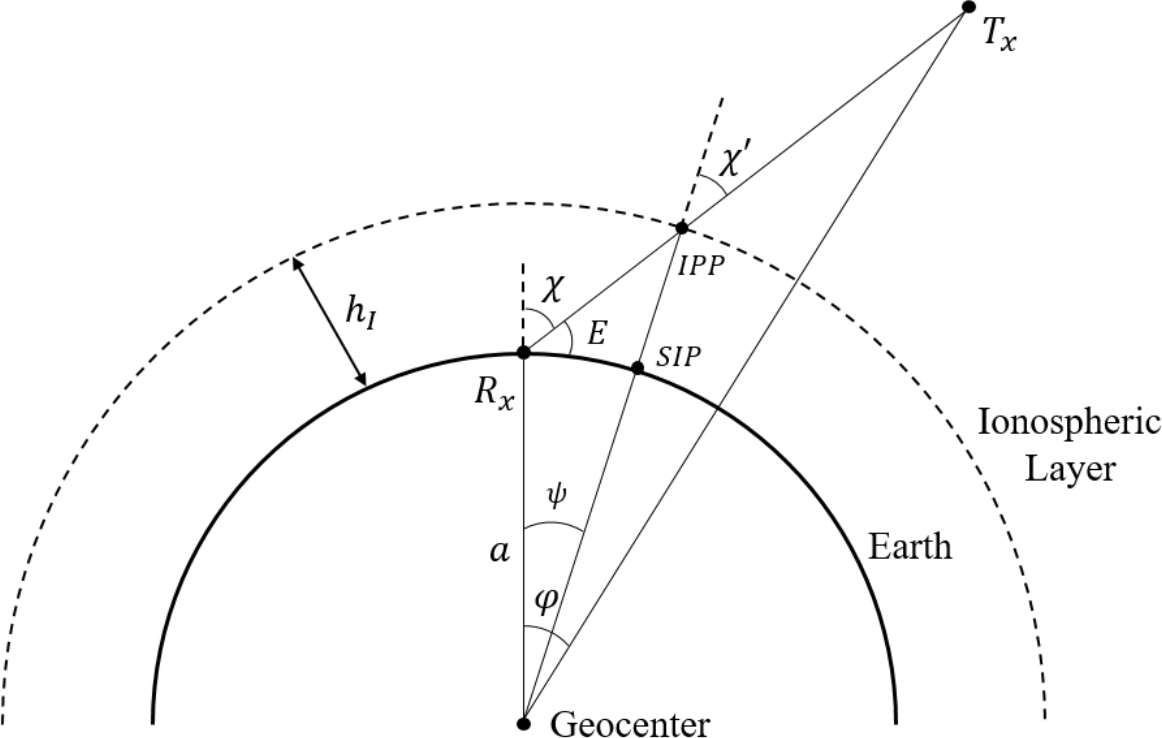
\includegraphics[width=0.7\linewidth]{fig/slm.png}    
\caption{Геометрия однослойной модели ионосферы.}
\label{fig-slm}      
\end{figure}

В связи с тем, что почти все сигналы GPS распространяются под наклоном к приёмнику, то следует использовать не вертикальный TEC (Vertical TEC, VTEC), а наклонный TEC (Slant TEC, STEC), которые связаны между собой соотношением:
\begin{equation}
\text{STEC}=F\times\text{VTEC}
\label{eq-stec}
\end{equation}
где
$F=\text{sec}\,\chi'$ -- наклонный коэффициент.
STEC можно получить на основе двухчастотных кодовых \eqref{eq-pr} или фазовых \eqref{eq-cr2} измерений сигналов GPS \cite{Hofmann2008}:
\begin{equation}
\begin{aligned}
\text{STEC}&=\frac{1}{40,38}\frac{f_1^2f_2^2}{f_1^2-f_2^2}(R_1-R_2) \\
&=\frac{1}{40,38}\frac{f_1^2f_2^2}{f_1^2-f_2^2}\left[(\lambda_1\Phi_1-\lambda_2\Phi_2)-(\lambda_1N_1-\lambda_2N_2)\right] 
\end{aligned}
\end{equation}

В модели Клобучара средняя высота ионосферы $h_I$ принимается равной 350 км, а $F$ выражается через угол места $E=90-\chi$.
Поэтому $F$ можно переписать как:
\begin{equation}
F=\text{sec}\left[\text{arcsin}(0,95\cos E)\right]
\end{equation}
Выполнение тригонометрических операций требует больших вычислительных затрат, чем для арифметических.
Поэтому для повышения скорости алгоритма Клобучара, наклонный коэффициент $F$ аппроксимируется следующим образом:
\begin{equation}
F\approx1+2\left(\frac{95-E}{90}\right)^3
\label{eq-slant-factor}
\end{equation}
Такое приближение даёт погрешность наклонного коэффициента $F$ в пределах 2\% для всех углов места больше 5\degree. 

Другой величиной, используемой в алгоритме Клобучара, является геоцентрических угол $\psi$ между приёмником и IPP.
$\psi$ можно  выразить, как функцию угла места $E$.
Для этого на рис. \ref{fig-slm} рассмотрим треугольник c вершинами в геоцентре, $R_x$ и IPP.
Сумма углов любого треугольника равна 180\degree:
\begin{equation}
90+E+\chi'+\psi=180    
\end{equation}
С учётом выражения \eqref{eq-zenith-angle} получается:
\begin{equation}
\psi=90-E-\text{arcsin}\left(\frac{a}{a+h_I}\sin\chi\right)   
\end{equation}
И наконец, аппроксимируя тригонометрические функции, приходим к:
\begin{equation}
\psi\approx\frac{445}{E+20}-4
\label{eq-geocentric angle}
\end{equation}
Такое приближение даёт погрешность геоцентрического угла $\psi$ в пределах 0,2\degree~для всех углов места больше 10\degree~и 0,5\degree~для всех углов места меньше 10\degree.

Приёмники GPS обычно имеют некоторую оцентку своих текущих геодезических координат: широты $\phi_u$ и долготы $\lambda_u$.
Однако в однослойной модели ионосферы групповая задержка сигнала измеряется в ионосферной точке, геодезические координаты которой для наклонных трасс распространения будут другими.
Вертикальная проекция IPP на поверхность Земли называется подионосферной точкой (Sub-Ionospheric Point, SIP).
Широта $\phi_I$ и долгота $\lambda_I$ подионосферной точки могут быть выражены следующим образом:
\begin{equation}
\begin{gathered}
\phi_I=\text{arcsin}(\sin \phi_u\cos \psi+\cos\phi_u\sin\psi\cos A) \\
\lambda_I=\lambda_u+\text{arcsin}\left(\frac{\sin\psi\sin A}{\cos\phi_I}\right)
\end{gathered}    
\end{equation}
где
$A$ -- азимутальный угол, измеренный относительно географического северного полюса.
На коротких расстояниях кривизна Земли незначительна, поэтому целесообразно использовать приближение плоской Земли, которое упрощает выражения выше:
\begin{equation}
\begin{gathered}
\phi_I\approx\phi_u+\psi\cos A \\
\lambda_I\approx\lambda_u+\frac{\psi\sin A}{\cos\phi_I}
\end{gathered}  
\label{eq-lat-lon-sip}  
\end{equation}
Такие приближения удовлетворительны для всех широт меньше 75\degree.
В алгоритме Клобучара широты, которые больше 75\degree, просто определяются равными 75\degree, чтобы избежать больших ошибок.

TEC и, следовательно, групповая задержка сигнала, строго говоря, зависят не от географической широты, а от геомагнитной.
Поэтому алгоритм Клобучара включает в себя преобразование геодезической широты в геомагнитную:
\begin{equation}
\sin\phi_m=\sin\phi\sin\phi_p+\cos\phi\cos\phi_p\cos(\lambda-\lambda_p)
\end{equation}
где
$\phi_m$ -- геомагнитная широта;
$\phi$ и $\lambda$ -- геодезические координаты, которые необходимо преобразовать;
$\phi_p$ и $\lambda_p$ -- геодезические координаты северного геомагнитного полюса Земли.
В модели Клобучара $\phi_p=78,3\degree$ и $\lambda_p=291\degree$.
Поэтому приближение $\phi_m$ в градусах имеет следующий вид:
\begin{equation}
\phi_m=\phi+11,6\cos(\lambda-291)
\label{eq-geomag-lat}
\end{equation}
Такое приближение даёт погрешность геомагнитной широты $\phi_m$ в пределах 1\degree~для всех широт меньше 40\degree~и 2\degree~для широт меньше 65\degree. 
Следует отметить, что геомагнитный северный полюс Земли со временем мигрирует, поэтому его текущие координаты больше не совпадают с теми, которые используются в модели Клобучара. 
Согласно модели IGRF-12 \cite{Thebault2015} в 2017 году координаты северного геомагнитного полюса составляли $\phi_p=80,4\degree$ и $\lambda_p=287,2\degree$.
Однако влияние этого эффекта на расчёт геомагнитной широты незначительно и вносит погрешность в уравнение \eqref{eq-geomag-lat} не более 2,1\degree.

При своих вычислениях алгоритм Клобучара использует местное время в SIP, которое может быть найдено в единицах часов на основе геодезической долготы и всемирного координатного времени UTС:
\begin{equation}
t=\frac{\lambda_I}{15}+t_{UTC}
\label{eq-sip-time}
\end{equation}
где
$t_{UTC}$ -- вcемирное координатное время в единицах часов.  

Резюмируя написанное выше, можно преступить к непосредственному описанию работы алгоритма Клобучара.
Модель Клобучара для вертикальной групповой ионосферной задержки сигнала $I_V$ математически записывается как:
\begin{equation}
I_V=DC+A\cos\left(\frac{2\pi(t-t_0)}{P}\right)  
\label{eq-vion-delay}
\end{equation}
где 
$DC=5$ нс -- постоянная (ночная) составляющая вертикальной групповой ионосферной задержки для сигнала L1;
$A$, $P$ и $t_0=14$ часов -- амплитуда, период и начальная фаза (без учёта $2\pi$) дневной функции косинуса.
Аналогично выражению \eqref{eq-stec}, наклонная групповая ионосферная задержка сигнала будет равна:
\begin{equation}
I=F\times I_V
\label{eq-sion-delay}
\end{equation}

Приёмник GPS имеет следующие входные параметры: собственные приблизительные геодезические координаты $\phi_u$ и $\lambda_u$, азимутальный угол $A$ и восемь коэффициентов модели Клобучара $\alpha_n$ и $\beta_n$ ($n=0,1,2,3$).
Стоит отметить, что при всех дальнейших выкладках углы полагаются безразмерными и кратными 180\degree, т.е. измеряются в полукругах, а время -- в секундах.
Алгоритм Клобучара включает в себя следующие шаги:
\begin{enumerate}
\item Согласно \eqref{eq-geocentric angle}, вычисляется угол между приёмником и IPP:
\begin{equation}
\psi=\frac{0,0137}{E+0,11}-0,022
\end{equation}
\item Согласно \eqref{eq-lat-lon-sip}, вычисляются широта и долгота SIP:
\begin{equation}
\begin{gathered}
\phi_I=\begin{cases}
0,416,&\phi_I>0,416 \\
\phi_u+\psi\cos A,&0,416\leqslant\phi_I\leqslant 0,416\\
-0,416,&\phi_I<0,416
\end{cases} \\
\lambda_I=\lambda_u+\frac{\psi\sin A}{\cos\phi_I}
\end{gathered}
\end{equation}
\item Согласно \eqref{eq-geomag-lat}, вычисляется геомагнитная широта SIP:
\begin{equation}
\phi_m=\phi_I+0,064\cos(\lambda_I-1,617)
\end{equation}
\item Согласно \eqref{eq-sip-time}, вычисляется местное время в SIP:
\begin{equation}
t=\begin{cases}
43200\lambda_I+t_{UTC}+86400,&t<0 \\
43200\lambda_I+t_{UTC},&0\leqslant t\leqslant 86400 \\
43200\lambda_I+t_{UTC}-86400,&t>86400    
\end{cases}
\end{equation}
\item На основе коэффициентов $\alpha_n$ и $\beta_n$ вычисляются амплитуд, период и фаза дневной функции косинуса \eqref{eq-vion-delay}:
\begin{equation}
\begin{aligned}
&A=\begin{cases}
\sum\limits_{n=0}^3\alpha_n\phi_m^n,&A\geqslant 0 \\
0,&A<0 
\end{cases} \\
&P=\begin{cases}
\sum\limits_{n=0}^3\beta_n\phi_m^n,&P\geqslant 72000 \\
72000,&P<0 
\end{cases} \\
&X=\frac{2\pi(t-50400)}{P}   
\end{aligned}
\end{equation}
\item Согласно \eqref{eq-slant-factor}, вычисляется наклонный коэффициент:
\begin{equation}
F=1+16(0,53-E)^3
\end{equation}
\item Согласно \eqref{eq-sion-delay}, приближённо вычисляется наклонная групповая ионосферная задержка сигнала:
\begin{equation*}
I=\begin{cases}
F\left[5\times10^{-9}+\sum\limits_{n=0}^3\alpha_n\phi_m^n\left(1-\frac{X^2}{2}+\frac{X^4}{24}\right)\right],&|X|\leqslant1,57 \\
5\times10^{-9},&|X|>1,57
\end{cases}
\end{equation*}
\end{enumerate}

Стоит ещё раз упомянуть, что полученная ионосферная задержка соответствует только сигналу L1.
Однако с её помощью можно довольно просто получить задержки, которые испытывают сигналы на других частотах:
\begin{equation}
I_f=\left(\frac{f_{L1}}{f}\right)^2I_{L1}
\end{equation}

Как итог, модель Клобучара способна устранить ионосферную ошибку примерно на 50\%. 